\chapter{Capa de usuario}

Inicialmente, el sistema en su forma gráfica fue pensado sólo como una interfaz de dos partes: una básica (Img.~\ref{img:basicQuery}) y una avanzada (Img.~\ref{img:advancedQuery}), lo cual fue con tiempo evolucionando.

\begin{figure}[ht!]
	\centering
	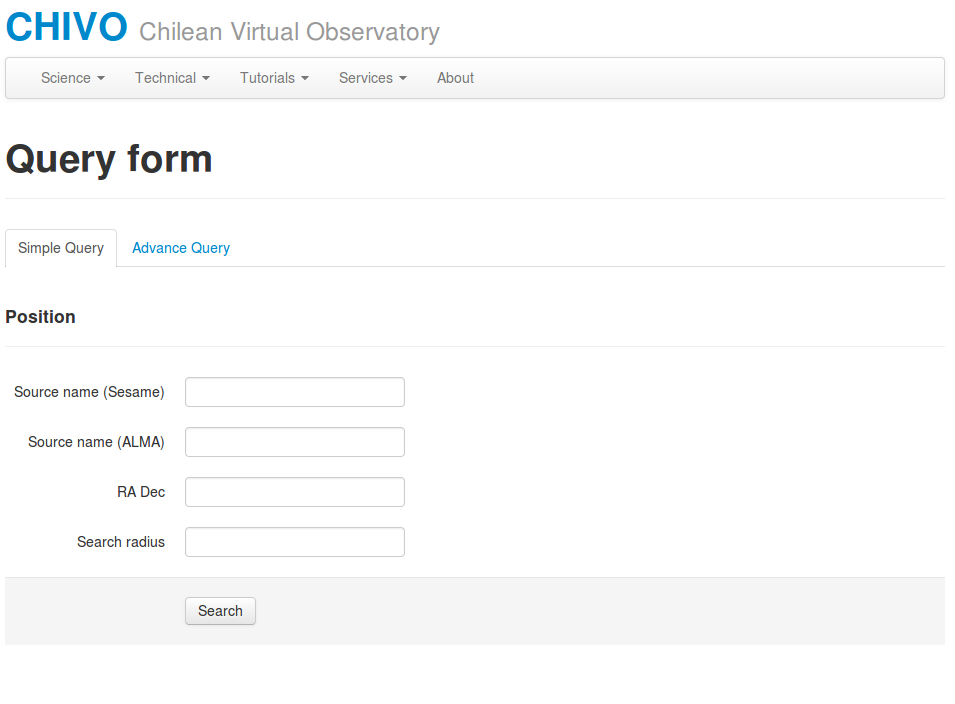
\includegraphics[scale=.4]{basicQuery}
	\caption{Maqueta inicial para búsqueda básica.}
	\label{img:basicQuery}
\end{figure}

\begin{figure}[ht!]
	\centering
	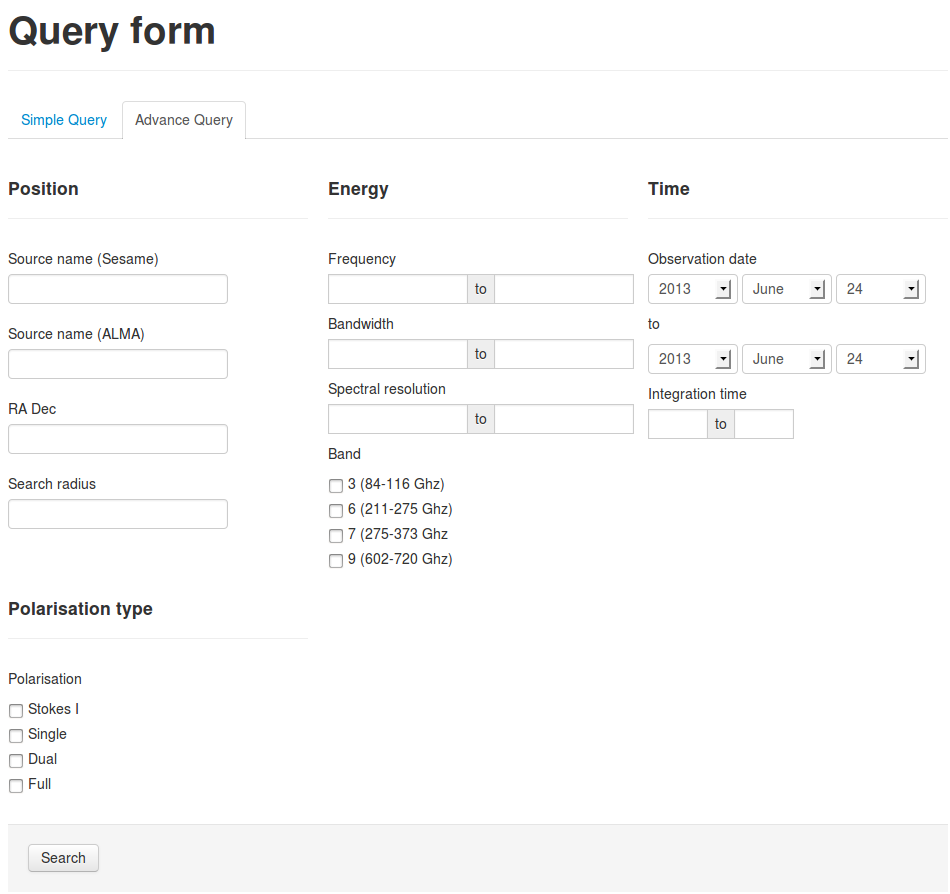
\includegraphics[scale=.4]{advancedQuery}
	\caption{Maqueta inicial para búsqueda avanzada.}
	\label{img:advancedQuery}
\end{figure}
